\documentclass[spanish, 10pt,a4paper]{article}
\usepackage[spanish]{babel}
\usepackage[utf8]{inputenc}
\usepackage{textcomp}
\usepackage{hyperref}
\usepackage[pdftex]{graphicx}
\usepackage{epsfig}
\usepackage{amsmath}
\usepackage{hyperref}
\usepackage{amssymb}
\usepackage{color}
\usepackage{graphics}
\usepackage{clrscode3e}
\usepackage{amsthm}
\usepackage{subcaption}
\usepackage{caratula}
\usepackage{fancyhdr,lastpage}
\usepackage[paper=a4paper, left=1.4cm, right=1.4cm, bottom=1.4cm, top=1.4cm]{geometry}
\usepackage[table]{xcolor} % color en las matrices
\usepackage[font=small,labelfont=bf]{caption} % caption de las figuras en letra mas chica que el texto
\usepackage[ruled,vlined,linesnumbered]{algorithm2e}
\usepackage{listings}
\usepackage{float}
\usepackage{amsfonts}
\usepackage{upgreek}


\color{black}

%%%PAGE LAYOUT%%%
\topmargin = -1.2cm
\voffset = 0cm
\hoffset = 0em
\textwidth = 48em
\textheight = 164 ex
\oddsidemargin = 0.5 em
\parindent = 2 em
\parskip = 3 pt
\footskip = 7ex
\headheight = 20pt
\pagestyle{fancy}
\lhead{AyED	 III - 2014 C2 - Trabajo Pr\'actico 2} % cambia la parte izquierda del encabezado
\renewcommand{\sectionmark}[1]{\markboth{#1}{}} % cambia la parte derecha del encabezado
\rfoot{\thepage}
\cfoot{}
\numberwithin{equation}{section} %sets equation numbers <chapter>.<section>.<subsection>.<index>

%Lo siguiente controla el ancho de las figuras (principalmente para el texto de los captions)
%\newcommand{\figurewidth}{.9\textwidth}
\newcommand{\figurewidth}{1\textwidth}

\newcommand{\tuple}[1]{\ensuremath{\left \langle #1 \right \rangle }}
\newcommand{\Ode}[1]{\small{$\mathcal{O}(#1)$}}
\newtheorem{teorema}{Teorema}[section]


%El siguiente paquete permite escribir la caratula facilmente
\hypersetup{
  pdftitle={ AyED III - TP1 },
  colorlinks,
  citecolor=black,
  filecolor=black,
  linkcolor=black,
  urlcolor=black 
}

\materia{Algoritmos y Estructuras de Datos III}

\titulo{Trabajo Práctico 1}

\subtitulo{Informe y análisis de resultados.}

\grupo{Grupo Theta}

\integrante{Rey, Martin}{483/12}{marto.rey2006@gmail.com}
\integrante{Marta, Cristian Gabriel}{079/12}{cristiangmarta@gmail.com}
\integrante{Lebedinsky, Alan}{802/11}{alanlebe@gmail.com}
\integrante{Coronel, Ezequiel}{352/08}{ecoronel@dc.uba.ar}
 
\begin{document}
{ \oddsidemargin = 2em
	\headheight = -20pt
	\maketitle
}
	\tableofcontents
	\newpage
	\section*{Introducción}
\addcontentsline{toc}{section}{Introducci\'on}

En el presente trabajo práctico se intenta resolver mediante algoritmos ciertos problemas brindados por la c\'atedra. 
Se decidi\'o implementar dichas soluciones usando el lenguaje \textit{C++}\cite{cplusplus}. Junto con las implementaciones, se adjunta el presente 
informe que especifica los detalles sobre el desarrollo de las soluciones, as\'i como pruebas, 
cálculos de complejidad temporal, mediciones, etc.\\
Para calcular la complejidad de los algoritmos involucrados, utilizamos el \textbf{modelo de costos uniforme}, que es el solicitado por el enunciado.

	\newpage
	\section{Problema 1: Plan de vuelo}

\subsection{Introducci\'on}
Una empresa nacional en la cual la presidenta está involucrada, nos contrató para resolver un problema el cual creen les hará ganar mucho dinero \textbf{legal}.
El problema consiste en agregarle una nueva funcionalidad al sitio web de la empresa tal que el usuario pueda seleccionar 
una ciudad \textbf{A} como origen y otra ciudad \textbf{B} como destino. Esta generará el itinerario de vuelos entre 
la ciudad \textbf{A} y la ciudad \textbf{B}. Para ello se cuenta con \textbf{n} distintos vuelos. De cada vuelo se conoce la ciudad de origen, la ciudad de destino, el momento de la partida y el momento de la llegada. Los momentos de partida y llegada representan la cantidad horas transcuridas desde que el usuario
realizó la consulta. El itenerario de vuelos deberá iniciar en la ciudad \textbf{A} y llegar a la ciudad \textbf{B} los antes posible.\\

Por ejemplo, el usuario quiere ir de \textbf{Rosario} a \textbf{Madrid}. Al momento de la consulta, se cuenta con sólo 6 vuelos. 
Lo siguiente es la entrada que recibirá nuestro problema:

\begin{codebox}
Rosario Madrid 6\\
Rosario Buenos\_Aires 2 3\\
Buenos\_Aires Madrid 6 18\\
Buenos\_Aires Madrid 7 20\\
Rosario San\_Pablo 3 6\\
San\_Pablo Madrid 8 17\\
San\_Pablo Madrid 7 16
\end{codebox}

Por ejemplo, existe un vuelo para ir desde Rosario a San Pablo que parte en 3hs y llega en 6hs posterior al momento de realizada la consulta. Otro vuelo disponible es ir de San Pablo a Madrid y parte dentro de 8hs y arribará dentro de 17hs a Madrid.\\

Dada esta instancia del problema, para ir desde Rosario y llegar a Madrid lo antes posible, la solución óptima sería tomar el vuelo de Rosario a San Pablo y luego el vuelo a Madrid (el que parte 8hs y arribará 17hs), llegando a destino 17hs luego de realizada la consulta. \\

Este es un ejemplo de salida de nuestro algoritmo:
\begin{codebox}
17 2 4 5
\end{codebox}

Cabe destacar, que debe haber una diferencia de 2hs entre la llegada de un vuelo y el horario de partida del próximo vuelo en el itinerario. Por tal motivo, en la solución óptima propuesta, el vuelo número 6 no fue considerado y se utilizó el vuelo número 5.

\newpage
\subsection{Desarrollo}

Dado que el problema trata de minimizar una magnitud (la cantidad de horas transcurridas desde realizada la consulta), nuestra primera idea fue 
modelar tal problema como un grafo y luego tratar de utilizar un algoritmo de camino mínimo como Dijsktra. En realidad, una variación de dicho
algoritmo adaptado al problema en cuestión. A continuación describiremos como modelaremos el problema con un grafo $G$.\\

\textbf{Vértices:} Serán las distintas ciudades existentes en el listado de vuelos. Ejemplo: Rosario, Lima, Bogotá, etc.\\
\indent
\textbf{Aristas:} Conetaremos las ciudades con los vuelos disponibles. Como tendremos aristas dirigidas (ciudad origen $\rightarrow$ ciudad destino), 
en principio $G$ será un grafo dirigido. 
Pero atención al siguiente detalle. Podríamos tener situaciones en las que existan mas de un vuelo con el mismo origen y destino. 
Entonces, por dicho motivo $G$ será un multigrafo (sin bucles) dirigido. \\

En la figura~\ref{ej1_grafo0} tenemos una representación gráfica de $G$ que incluye algunas ciudad de Asia y algunos posibles vuelos entre dichas ciudades.

\begin{figure}[h!]
  \centering
  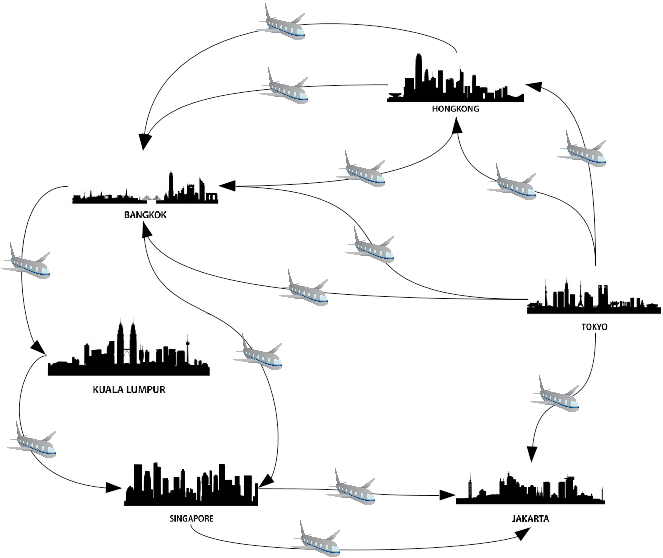
\includegraphics[scale=0.75]{Imagenes/ej1_grafo0}
  \caption{Ejemplo del grafo G con as ciudades como vértices y los vuelos como aristas}
  \label{ej1_grafo0}
\end{figure}

Ahora nos falta definir las magnitudes o valores asociados a las aristas (distancia) y el objetivo.\\

\indent
\textbf{Distancia:} Cada arista tendrá asociada la hora de llegada del vuelo, un valor entero no negativo que representa la cantidad de horas transcurridas desde el momento que se realizó la consulta. \\
\indent
\textbf{Objetivo:} Ir de un vértice (ciudad) a otro minimizando la distancia (la hora de llegada).\\

En la figura~\ref{ej1_grafo1} tenemos una representación del problema de ir desde \textbf{Tokyo} a 
\textbf{Singapore}  y queremos minimizar la hora de llegada. Las horas de llegadas se encuentran en las aristas (junto a los aviones).\\

\begin{figure}[h!]
  \centering
  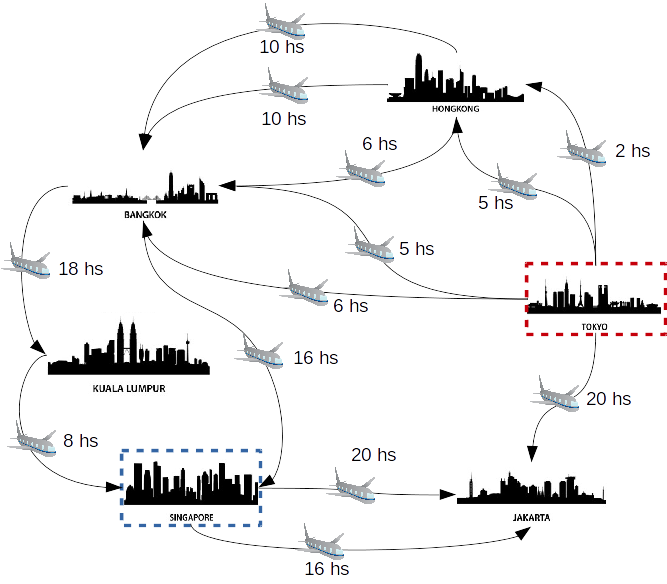
\includegraphics[scale=0.75]{Imagenes/ej1_grafo1}
  \caption{Ejemplo del grafo G para ir desde Tokyo a Singapore y llegar cuanto antes}
  \label{ej1_grafo1}
\end{figure}

\newpage
Ahora tenemos nuestro problema modelado como un problema de grafos. Pero nos están quedando algunas cosas afuera como por ejemplo 
la restricción de 2hs entre vuelo y vuelo. Otro detalle al que hay que prestar atención es que si a este grafo $G$ le aplicamos al 
algoritmo de camino mínimo de Dijsktra no nos va a dar la mínima hora de llegada al destino final. 
Entonces, para solventar estos 2 obstaculos que acabamos de encontrar realizaremos 2 pequeños cambios en el algoritmo original (Algoritmo~\ref{Dijsktra}).

\LinesNumbered
\begin{algorithm}[H]
\DontPrintSemicolon
\KwData{\textbf{origen}: vértice, \textbf{destino}: vértice, \textbf{k}: cant. ciudades, \textbf{adyacencias}: vector de adyacencias}
\Begin{
	cola $\Leftarrow$ ColaPrioridad()\;
	distancia $\Leftarrow$ Vector()\;
    \For{ i $\in$ k } {
        distancia[i] $\Leftarrow \infty$ \;
    }
    distancia[origen] $\Leftarrow$ 0\;
    cola.agregar(tupla(origen, distancia[origen]))\;
    \While{! cola.vacia()} {
        u $\Leftarrow$ cola.minimo()\;
		\For{ v $\in$ adyacencias[u.prim] } {
			\If{ distancia[v.prim] $\ge$ distancia[u.prim] + v.terc}  {
                distancia[v.prim] $\Leftarrow$ distancia[u.prim] + v.terc\;
                cola.agregar(tupla(v, distancia[v.prim]))\;
			}
		}
    }
    \Return{distancia[destino]}
}
\caption{\textbf{Dijsktra } \label{Dijsktra}}
\end{algorithm}

El vector de adyacencias está indexado por la ciudad de origen y cada posición contiene una terna:\\
\textbf{prim}: Ciudad destino.\\
\textbf{segu}: Hora de partida.\\
\textbf{terc}: Hora de llegada.\\

En la cola prioridad (ordenada de menor a mayor) contiene tuplas, donde cada una contiene:\\
\textbf{prim}: Ciudad (actual).\\
\textbf{segu}: Hora de llegada.\\

El primer cambio que realizaremos en el algoritmo~\ref{Dijsktra} será en vez acumular la distancia mínima en el vector $distancia$ (línea 12), 
guardar la hora de llegada. Esto también nos obliga a modificar la línea 11 para ir guardando la hora mínima de llegada. De esta manera iremos
gurdando la hora mínima de llegada para cada ciudad alcanzable desde la ciudad $origen$ en el vector $distancia$. Cuando el algoritmo termine,
en la posición $destino$ del vector $distancia$ tendremos la hora mínima de llegada para la ciudad $destino$. En caso de no haber un camino, esta
posición tendrá $\infty$. \\

El siguiente cambio es la restricción de 2 horas entre vuelo y vuelo. Es decir, la hora de partida del próximo vuelo a tomar debe ser por lo menos
mayor o igual en 2 horas a la hora de llega del vuelo previo. Los próximo vuelos con cidad origen $u.prim$ son los $v \in adyacencias[u.prim]$. 
Como $v.segu$ es la hora de partida y $u.segu$ la hora de llegada (notar que también puede utilizar $distancia[u.prim]$), basta con agregar
la condición $distancia[u.prim] \le v.segu - 2$ dentro del bucle mas anidado antes de que actulice la distincia (línea 11, algoritmo~\ref{DijsktraMod})

\LinesNumbered
\begin{algorithm}[H]
\DontPrintSemicolon
\KwData{\textbf{origen}: vértice, \textbf{destino}: vértice, \textbf{k}: cant. ciudades, \textbf{adyacencias}: vector de adyacencias}
\Begin{
	cola $\Leftarrow$ ColaPrioridad()\;
	distancia $\Leftarrow$ Vector(k)\;
    \For{ i $\in$ k } {
        distancia[i] $\Leftarrow \infty$ \;
    }
    distancia[origen] $\Leftarrow$ 0\;
    cola.agregar(tupla(origen, distancia[origen]))\;
    \While{! cola.vacia()} {
        u $\Leftarrow$ cola.minimo()\;
		\For{ v $\in$ adyacencias[u.prim] } {
            \If{ distancia[u.prim] $\le$ v.segu - 2}  {
                \If{ distancia[v.prim] $\ge$ v.terc}  {
                    distancia[v.prim] $\Leftarrow$ v.terc\;
                    cola.agregar(tupla(v, distancia[v.prim]))\;
                }
            }
		}
    }
    \Return{distancia[destino]}
}
\caption{\textbf{DijsktraMod} \label{DijsktraMod}}
\end{algorithm}

\newpage
Al finalizar el algoritmo~\ref{DijsktraMod} devolverá la hora mínima de llegada a $destino$ saliendo desde $origen$. 
En el problema original nos solicitan saber los números de los vuelos, es decir, el itinerario de vuelos para llegar a destino cuanto antes.
Por tal motivo agregaremos algunas estructuras mas para poder reconstruir la solicitan. Agregaremos 2 vectores, uno para recordar al padre (ciudad) 
y otro para guarda el vuelo que le corresponde a dicha ciudad. Una vez que finaliza el bucle \textbf{while} y si este tiene una distancia que no sea
$\infty$, entonces agregamos al itinerario el vuelo que nos lleva a $destino$, es decir $vuelo[destino]$. 
Luego buscamos la $ciudad$ de la que partimos hacia destino con $padre[destino]$ y si esta ciudad es distinta de $origen$, entonces agrego el 
vuelo al itinerario. Nuevamente busco la ciudad de la que partí para llegar a $ciudad$ y si esta ciudad es distinta de $origen$, entonces agrego.
Repetimos esto hasta encontrar la ciudad $origen$.

\LinesNumbered
\begin{algorithm}[H]
\DontPrintSemicolon
\KwData{\textbf{origen}: vértice, \textbf{destino}: vértice, \textbf{k}: cant. ciudades, \textbf{adyacencias}: vector de adyacencias, \textbf{itinerario}: lista de vuelos}
\Begin{
	cola $\Leftarrow$ ColaPrioridad()\;
	distancia $\Leftarrow$ Vector(k)\;
	padre $\Leftarrow$ Vector(k)\;
	vuelo $\Leftarrow$ Vector(k)\;
    \For{ i $\in$ k } {
        distancia[i] $\Leftarrow$ padre[i] $\Leftarrow$ vuelo[i] $ \Leftarrow \infty$ \;
    }
    distancia[origen] $\Leftarrow$ 0\;
    cola.agregar(tupla(origen, distancia[origen]))\;
    \While{! cola.vacia()} {
        u $\Leftarrow$ cola.minimo()\;
		\For{ v $\in$ adyacencias[u.prim] } {
            \If{ distancia[u.prim] $\le$ v.segu - 2}  {
                \If{ distancia[v.prim] $\ge$ v.terc}  {
                    distancia[v.prim] $\Leftarrow$ v.terc\;
                    padre[v.prim] $\Leftarrow$ u.prim\;
                    vuelo[v.prim] $\Leftarrow$ v.id\;
                    cola.agregar(tupla(v, distancia[v.prim]))\;
                }
            }
		}
    }
    \If{ distancia[destino] $\ne \infty$ }  {
        itinerario.agregar(vuelo[destino])\;
        ciudad = padre[destino]\;
        \While{ciudad $\ne$ origen} {
            itinerario.agregar(vuelo[ciudad])\;
            ciudad = padre[destino]\;
        }
    }
    \Return{distancia[destino]}
}   
\caption{\textbf{DijsktraFinal} \label{DijsktraFinal}}
\end{algorithm}

\newpage
\subsection{Complejidad}
Para realizar el análisis de complejidad temporal utilizaremos el algoritmo~\ref{DijsktraFinal}. \\
La creación de la cola de prioridad vacía tiene una complejidad constante $c$. 
En cambio la creación e inicialización de los vectores tiene una complejidad de $k$ cada 1, entonces tenemos $3*k$ por la creación 
y $k$ para inicializar. Un acceso al vector y una asignación (línea 8), constante. Agregar un elemento a la cola de prioridad, en este caso particular
podemos considerarlo constante (porque la cola está vacía), no así mas adelante. Hasta aquí tenemos $4*k + c$.\\
Luego inicia un bucle while. Analicemos primero la complejidad del cuerpo del bucle y luego determinaremos cuantas veces se ejecuta. 
Extraer el mínimo elemento de la cola de prioridad tiene una complejidad logarítmica\cite{priorityQueuePop} en la cantidad de elementos de la cola. 
En el peor de los casos, la cola puede llegar a tener $k$ elementos (todas las ciudades), entonces, en el peor caso es $log\ k$. Esto también
nos dice que el bucle $while$ se ejecutará $k$ veces. Hasta aquí tenemos: $(4*k + c) + (k*log\ k)$.
Ahora nos agregar la complejidad del bucle $for$.
Como este bucle se va a ejecutar 1 vez para cada ciudad y para cada una se recorren sus vuelos, al final de todo se van a recorrer todos los vuelos.
Es decir que se va a ejecutar $n$ veces.
En el cuerpo del bucle $for$ hay varias comparaciones y asignaciones, las cuales podemos considerar
de complejidad constante. No sucede lo mismo con el agregar a la cola de prioridad que en el peor caso tiene $k$ elementos, lo que nos deja
una complejidad de $log\ k$. Entonces el bucle tiene una complejidad en el peor caso de $n*log\ k$. 
Esto nos deja la complejidad por ahora en: $(4*k + c) + (k*log\ k) + (n*log\ k)$.\\
Por último y no menos importante, falta analizar como se reconstruye la solución. Esta parte es sencilla, ya que si hay una solución, se agregan 1 a 1
los vuelos a una lista, agregar es constante y en el peor de los casos agrego los $n$ vuelos.\\
La complejidad nos queda en: $(4*k + c) + (k*log\ k) + (n*log\ k) + (n+c) = k*(log\ k) + n*(log\ k) + 4*k + n + 2*c$.\\

Veamos que $k$ (la cantidad de ciudades) está acotado por $n$ (la cantidad de vuelos). A lo sumo puedo tener $2*n$ ciudades distintas (2 por cada vuelo).\\
Dicho esto, nos queda: $2*n*(log\ 2*n) + n*(log\ 2*n) + 4*2*n + n + 2*c = 3*n*(log\ n) + 3*n*(log\ 2) + 9*n + 2*c$. Es decir $O(n*(log\ n))$.


\subsection{Testing}
En el archivo ej1/tester.cpp escribimos varios casos de prueba que nuestro algoritmo debía pasar.\\

El primer caso es para probar la restricción de 2hs entre vuelo y vuelo. Queremos ir desde Rosario a Madrid y llegar cuanto antes.

\begin{codebox}
Rosario Madrid 6\\
Rosario Buenos\_Aires 2 3\\
Buenos\_Aires Madrid 6 18\\
Buenos\_Aires Madrid 7 20\\
Rosario San\_Pablo 3 6\\
San\_Pablo Madrid 8 17\\
San\_Pablo Madrid 7 16\\
\end{codebox}

El vuelo que llega antes a Madrid es el 6 pero no podemos tomarlo debido a que llegaríamos a a San Pablo desde Rosario a las 6 (vuelo 4) y como debemos esperar
2 horas hasta tomar el próximo vuelo, debemos tomar el vuelo número 5. La salida de nuestro programa debería ser:
\begin{codebox}
17 2 4 5
\end{codebox}

Ahora, tenemos otro caso de prueba. Tenemos 10 vuelos disponibles para ir de Rosario a Paris y llegar cuanto antes.

\begin{codebox}
Rosario Paris 10\\
Rosario Buenos\_Aires 2 3\\
Buenos\_Aires Madrid 6 18\\
Buenos\_Aires Madrid 7 20\\
Rosario San\_Pablo 3 6\\
San\_Pablo Madrid 8 17\\
San\_Pablo Madrid 7 16\\
Madrid Paris 17 19\\
Barcelona Paris 19 20\\
Madrid Paris 18 20\\
Madrid Paris 19 20\\
\end{codebox}

Noten que la mayoría de los vuelos que arriban a Paris lo hacen em 20hs salvo 1 que lo hace en 19hs, procedente de Madrid pero para llegar a tomar
ese vuelo deberíamos llegar a Madrid cuando mucho en 15hs y no hay ningún vuelo que cumpla eso. Queda descartado. Vamos de Rosario a San Pablo 
y luego a Madrid (vuelos 4 y 5). Desde Madrid sólo tenemos una posibilidad (vuelo 10).

\begin{codebox}
20 3 4 5 10\\
\end{codebox}

Por último, un caso en el que no existe solución. Tengo 4 vuelos disponibles para ir de Rosario a Madrid.
\begin{codebox}
Rosario Madrid 4\\
Rosario Buenos\_Aires 2 3\\
Rosario San\_Pablo 3 6\\
San\_Pablo Barcelona 8 17\\
Barcelona Madrid 7 16\\
\end{codebox}

Para salir de Rosario tengo 2 vuelos: ir a Buenos Aires o ir a San Pablo. Desde Buenos Aires no hay vuelos, mientras que desde San Pablo puedo 
tomar el vuelo a Barcelona. Pero una vez en Barcelona no hay vuelos que me lleven a Madrid, pues llegaría a Barcelona en 17hs y el vuelo a Madrid 
sale en 7hs. Para este caso no hay solución y nuestro programa debería imprimir:
\begin{codebox}
no\\
\end{codebox}

\subsection{Experimentación}

Para la experimentación decidimos tomar ciertos conjuntos de datos. Los conjuntos de datos se caracterizan de la siguiente manera:\\

\textbf{k = n/2:} La cantidad de ciudades distintas (k) es alrededor la mitad de la cantidad de vuelos (n).\\
\indent \textbf{k = n:} La cantidad de ciudades distintas (k) es aproximadamente igual cantidad de vuelos (n).\\
\indent \textbf{k = 2n:} La cantidad de ciudades distintas (k) es alrededor el doble de la cantidad de vuelos (n).\\

La medición de tiempo se realizó de la siguiente manera: Para cada instancia/problema, se ejecutó 50 veces el algoritmo sobre dicha instancia,
acumulando los tiempos utilizando la biblioteca chrono. Luego se dividió el tiempo acumulado en 50, para tener un promedio del tiempo.

\begin{figure}[H]
  \centering
  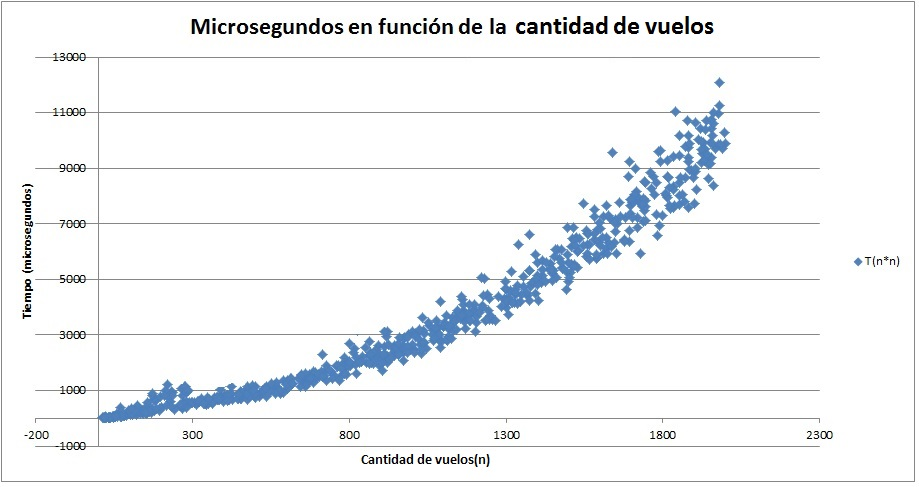
\includegraphics[scale=0.75]{Imagenes/Ej1/nSobre2}
  \caption{T(n$^{2}$) = tiempos  n vuelos. Estos resultados son para el conjunto de datos $k = n/2$.
      La curva tiene un forma cuadrática en función de la cantidad de vuelos. Para poder confirmar esto, en el siguiente gráfico dividiremos
    por $n^2$.
  }
  \label{}
\end{figure}

\begin{figure}[H]
  \centering
  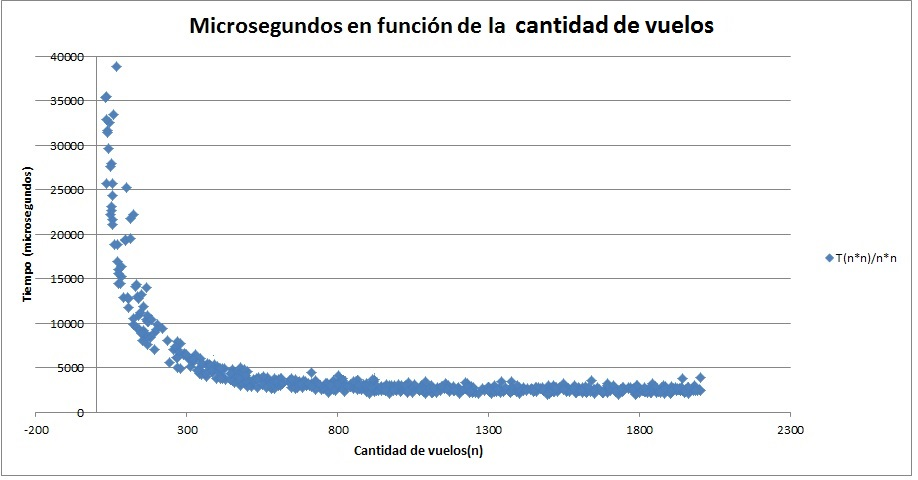
\includegraphics[scale=0.75]{Imagenes/Ej1/nSobre2Const}
  \caption{T(n$^{2}$) = tiempo para n vuelos. Esta figura es el resultado de dividir los tiempos de la gráfica anterior por $n^2$.
    Aquí se puede ver como estos resultados están acotados por una constante y parecería que continua decreciendo.  }
  \label{}
\end{figure}

\begin{figure}[H]
  \centering
  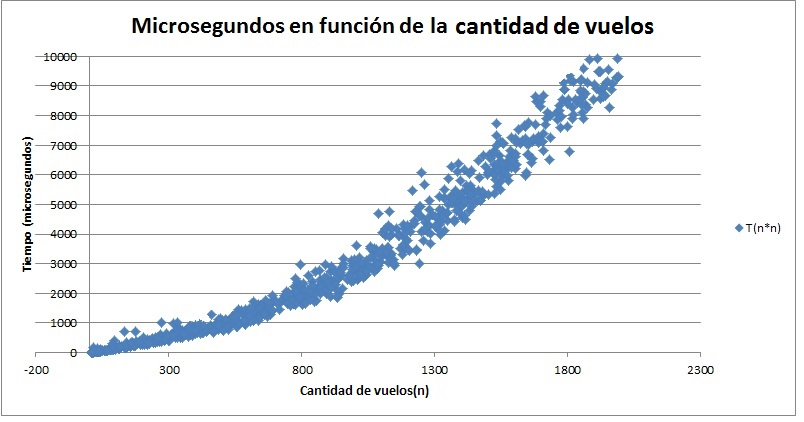
\includegraphics[scale=0.75]{Imagenes/Ej1/n}
  \caption{T(n$^{2}$) = tiempo para n vuelos. Estos resultados son para el conjunto de datos $k = n$. 
  Para este caso, la curva no parece ser tan pronunciada como en el caso anterior, que se parecía a $n^2$. 
  Una vez mas volveremos a dividir por $n^2$.}
  \label{}
\end{figure}

\begin{figure}[H]
  \centering
  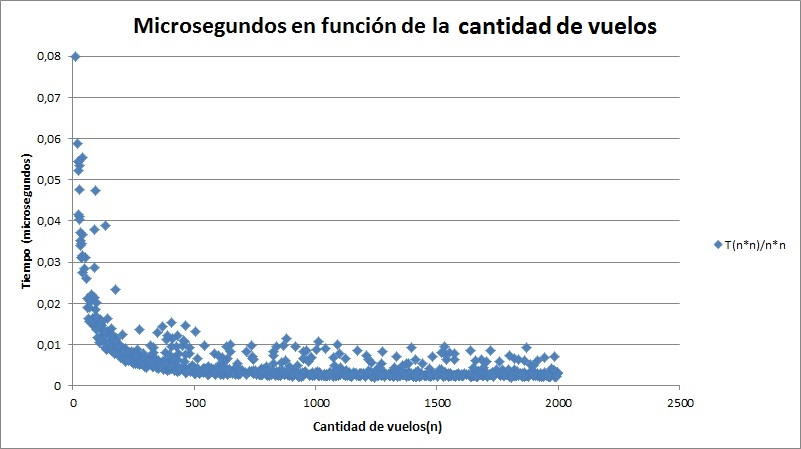
\includegraphics[scale=0.75]{Imagenes/Ej1/nConst}
  \caption{T(n$^{2}$) = tiempo para n vuelos. Esta figura es el resultado de dividir los tiempos de la gráfica anterior por $n^2$.
    Nuevamente podes apreciar que los resultados están acotados por una constante y otra vez parecería que continua decreciendo.}
  \label{}
\end{figure}

\begin{figure}[H]
  \centering
  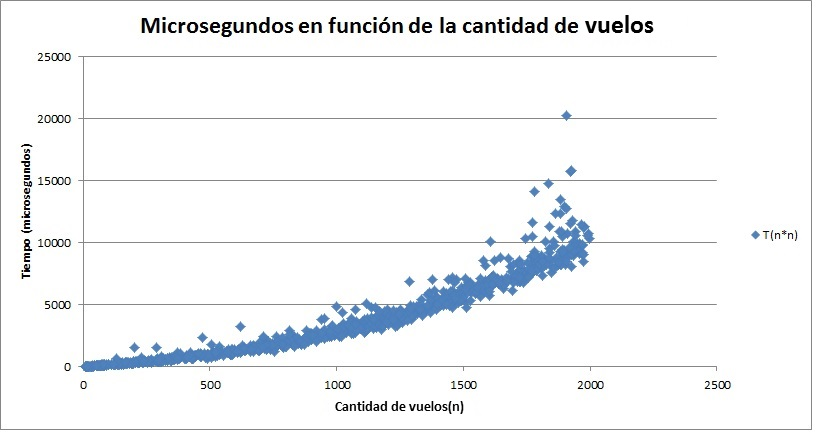
\includegraphics[scale=0.75]{Imagenes/Ej1/2n}
  \caption{T(n$^{2}$) = tiempo para n vuelos. Estos resultados son para el último conjunto de datos $k = 2n$. 
  En este caso, vemos que los resultados tienen una forma mas parecida a una recta con una leve inclinación. 
  Bastante distinto a los 2 primeros conjuntos de datos propuestos. Salvo una leve alteración en n=200 (la cual no pudimos analizar),
  el gráfico es bastante ser uniforme. Por último, dividiremos por $n^2$ los resultados en busca de la comstante.}
  \label{}
\end{figure}

\begin{figure}[H]
  \centering
  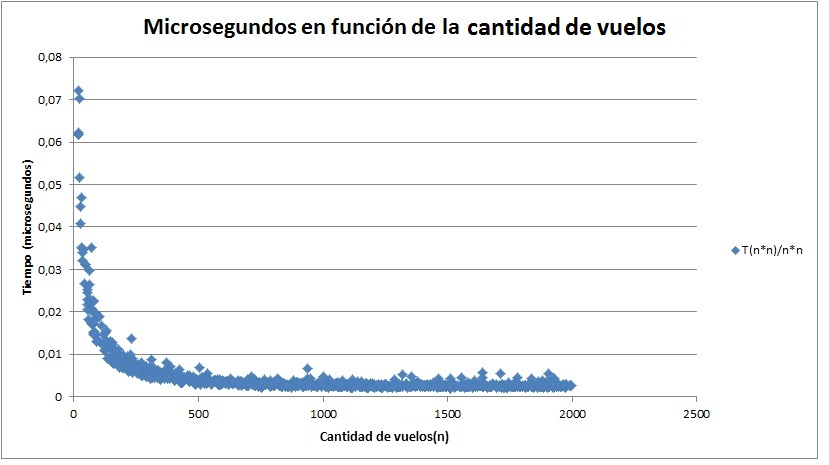
\includegraphics[scale=0.75]{Imagenes/Ej1/2nConst}
  \caption{T(n$^{2}$) = tiempo para n vuelos. Esta figura es el resultado de dividir los tiempos de la gráfica anterior por $n^2$.
    En este último gráfico, podemos ver la constante con un leve decrecimiento.}
  \label{}
\end{figure}


\subsection{Conclusión}
Dado el problema del plan de vuelo, lo modelamos con un multigrafo (sin bucles) dirigido y mediante una modificación 
del algoritmo de camino mínimo de Dijsktra pudimos resolverlo. En el análisis teórico de complejidad temporal concluimos
que el peor caso estaba en $O(n*(log\ n)$ pero durante la experimentación computacional, los datos empíricos nos mostraron
que nuestro algoritmo que con ciertos conjuntos de datos tiene un comportamiento cuadrático. Cabe destacar que aún así,
sigue respetando la exigencia del problema, que la solución debía ser no peor que $O(n^2)$.


	\newpage
	\section{Problema 2: Caballos salvajes}

\subsection{Introducci\'on}
La misma empresa nacional del anterior problema ahora quiere incursionar en el negocio de los juegos de mesa, por ello han sacado un innovador juego que utiliza un tablero cuadrado de ajedrez (hay en distintos tamaños) en donde se colocan en algunas casillas caballos blancos de ajedrez. El juego permite que haya mas de un caballo en la misma casilla, y los caballos pueden moverse por el tablero como lo harían en el ajedrez. Para ganar el juego hay que lograr ubicar a todos los caballos en una misma casilla en la menor cantidad total de movimientos posibles, es decir que la suma de los movimientos de todos los caballos en el tablero sea la menor. \\
A continuación se muestra un ejemplo del juego con su respectiva solución: \\

%\begin{figure}[h]
%  \centering
%    \includegraphics[scale=5]{Imagenes/introCaballos}
%  \caption{}
%  \label{fig:ejemplo}
%\end{figure}
%
%
%\begin{figure}[h]
%  \centering
%    \includegraphics[scale=5]{Imagenes/introSolu}
%  \caption{}
%  \label{fig:ejemplo}
%\end{figure}

\begin{figure}[H]
  \centering
		\begin{subfigure}[b]{0.3\textwidth}
                \includegraphics[scale=3]{Imagenes/Ej2/introCaballos}
                \caption{Inicio del juego}
                \label{fig:intro}
        \end{subfigure} 
  		\begin{subfigure}[b]{0.3\textwidth}
               \includegraphics[scale=3]{Imagenes/Ej2/introSolu}
                \caption{Solucion al juego}
                \label{fig:intro}
        \end{subfigure}
        \caption{Aunque no es visible en (b) se encuentran los dos caballos en el mismo casillero} 
\end{figure}


\subsection{Desarrollo}

Este problema lo resolvimos con una serie de pasos, primero comenzamos representando el tablero con el siguiente grafo: \\
Sea G(V,E) el grafo donde cada nodo v $\epsilon$ V representa una casilla del tablero y dos nodos $v_1$ y $v_2$ $\epsilon$ V están unidos por una arista e $\epsilon$ E $\Leftrightarrow$ es posible mover al caballo de la casilla $v_1$ a la casilla $v_2$. \\
Luego para cada caballo en su correspondiente casilla utilizamos el algoritmo de BFS sobre G, el cual para grafos con aristas no pesadas o de igual peso nos da el camino mínimo desde un nodo origen hasta cada uno del resto de los nodos del grafo \footnote{Cormen, T.,Leiserson, C.,Rivest,R.,Stein, C.,"Introduction to Algorithms", third edition, pagina 594}. Al algoritmo de BFS lo modificamos para que a medida que busca el camino mínimo a cada casilla calcule la cantidad de movimientos que le toma llegar a ésta casilla. \\
Después sumamos lo que le cuesta a cada caballo llegar a cada casilla obteniendo el total de movimientos que cuesta que todos los caballos lleguen a cada casilla. Finalmente nos quedamos con la casilla que lleguen todos los caballos y que haya resultado con menor cantidad total de movimientos. En caso que no haya ninguna casilla tal que todos los caballos lleguen a esta entonces la solución al problema será "no".



\begin{codebox}
\Procname{\textbf{Pseudoc\'odigo:}}
\li	creamos una matriz $acumMovimientos$ inicializada en 0
\li	creamos una matriz $cantidad$ inicializada en 0
\li	
\li	para cada caballo 
\li \ \ \	mientras recorremos G usando BFS desde la casilla donde se encuentra ubicado
\li	\ \ \ \ \ \		cantMov $\leftarrow$ contamos la cantidad de movimientos a cada casilla
\li	\ \ \ \ \ \		acumulamos en $acumMovimientos$ lo que contamos con cantMov
\li \ \ \	fin mientras
\li \ \ \	para cada casilla
\li	\ \ \ \ \ \		acumulamos en $cantidad$ si el caballo paso por esa casilla
\li \ \ \	fin para
\li	fin para
\li	
\li	buscar en $acumMovimientos$ la casilla que tenga menor cantidad de movimientos y que en $cantidad$
\li hayan pasado todos los caballos, retornar la casilla y la cantidad de movimientos
\li 
\li En caso que no existe tal casilla retornar "no"
\end{codebox}




\subsection{Demostraci\'on de correctitud} 

Antes que nada como nuestro algoritmo usa BFS, veamos que es correcto. Esto es cierto, ya que esta demostrado en el "Cormen" \footnote{Cormen, T.,Leiserson, C.,Rivest,R.,Stein, C.,"Introduction to Algorithms", third edition, pagina 594}. \\



Ahora para demostrar la correctitud de nuestro algoritmo vamos a usar inducción en n = cantidad de caballos. \\ \\

\textbf{Caso Base:} Queremos ver que nuestro algoritmo es correcto, es decir que nos da la solución óptima para 1 caballo, esto es fácil de ver pues el algoritmo aplicara BFS para calcular la cantidad de movimientos que le cuesta llegar al caballo a cada una de las casillas, y estos cálculos los guardara en la matriz $acumMovimientos$. Luego buscara en $acumMovimientos$ la casilla con menor cantidad de movimientos y se encontrara con que la casilla donde comenzó el caballo cuesta 0 (ya que no se movería) y devolvería esta casilla que costo 0 movimientos como resultado.\\

\textbf{Paso inductivo:} P(n) = nuestro algoritmo calcula correctamente en una matriz, para cada posición si llegan los n caballos y la cantidad de movimientos totales de los n caballos para llegar a tal posición.
Queremos ver que vale P(n+1), esto quiere decir que queremos ver que para n+1 caballos el algoritmo nos calcula correctamente la matriz con la cantidad de movimientos totales de cada casilla y la cantidad de caballos que pasan por cada casilla. \\

Por hipótesis inductiva vale P(n), veamos qué pasa cuando agregamos el n+1 caballo, el algoritmo recorrerá G (definido en la sección 2.2) usando BFS y para cada casilla contara la cantidad de movimientos. Una vez terminado el recorrido de BFS, se recorrerá el tablero para saber a qué casillas llega y la cantidad de movimientos a la casilla del n+1 caballo acumulando esto en lo que ya se tenía para los n caballos anteriores. Con esto terminaremos teniendo en una matriz el costo total de movimientos para cada casilla de los n+1 caballos y la cantidad de caballos que pasan por cada casilla, que es lo queríamos pues solo falta buscar la casilla donde hayan llegado todos los caballos y el costo total sea mínimo.






\newpage
\subsection{Complejidad}

A continuación el extracto más importante del código para analizar la complejidad: 

\begin{codebox}
\Procname{$\proc{\textbf{Caballos Salvajes}}$()}
\li matriz\_t acumMovimientos(n\_, vector$<$int$>$(n\_, 0)); 	\RComment{O(n$^{2}$)}
\li	matriz\_t cantidad(n\_, vector$<$int$>$(n\_, 0));			\RComment{O(n$^{2}$)}
\li	
\li	for(int cab = 0; cab $<$ k\_; ++cab) \{						\RComment{O(k*n$^{2}$)}
\li \ \ \		matriz\_t movimientos(n\_, vector$<$int$>$(n\_, 0));	\RComment{O(n$^{2}$)}
\li	\ \ \		bfs(caballos\_[cab], movimientos);				\RComment{O(n$^{2}$)}
\li
\li	\ \ \		for (int i = 0; i $<$ n\_; ++i) \{				\RComment{O(n$^{2}$)}
\li	\ \ \ \ \ \		for (int j = 0; j $<$ n\_; ++j) \{			\RComment{O(n)}
\li	\ \ \ \ \ \ \ \ \		acumMovimientos[i][j] += movimientos[i][j];	\RComment{O(1)}
\li	\ \ \ \ \ \ \ \ \		if (movimientos[i][j] $>$ 0) \{		\RComment{O(1)}
\li	\ \ \ \ \ \ \ \ \ \ \ \			++cantidad[i][j];			\RComment{O(1)}
\li	\ \ \ \ \ \ \ \ \		\} else \{
\li	\ \ \ \ \ \ \ \ \ \ \ \		if ( (caballos\_[cab].first-1 == i) \&\& (caballos\_[cab].second-1 == j)) \{								\RComment{O(1)}
\li	\ \ \ \ \ \ \ \ \ \ \ \ \ \ \		++cantidad[i][j];		\RComment{O(1)}
\li	\ \ \ \ \ \ \ \ \ \ \ \		\}
\li	\ \ \ \ \ \ \ \ \		\}
\li	\ \ \ \ \ \			\}
\li	\ \ \			\}
\li
\li	m\_ = numeric\_limits$<$int$>$::max();						\RComment{O(1)}
\li	for (int i = 0; i $<$ n\_; ++i) \{							\RComment{O(n$^{2}$)}
\li \ \ \	for (int j = 0; j $<$ n\_; ++j) \{					\RComment{O(n)}
\li	\ \ \ \ \ \	if (cantidad[i][j] == k\_) \{					\RComment{O(1)}
\li	\ \ \ \ \ \ \ \ \	m\_ = acumMovimientos[i][j];			\RComment{O(1)}
\li	\ \ \ \ \ \ \ \ \	f\_ = i+1;								\RComment{O(1)}
\li	\ \ \ \ \ \ \ \ \	c\_ = j+1;								\RComment{O(1)}
\li	\ \ \ \ \ \ 	\}
\li \ \ \		\}
\li			\}
\end{codebox}


Podemos ver que comienza creando 2 matrices de dimensiones n*n (líneas 1 y 2), lo cual demandara esa cantidad de operaciones O(n$^{2}$). Después hay un for (línea 4) que itera k veces y en cada iteración tiene que:

 \begin{itemize}
 \item	crear la matriz $movimientos$ (línea 5) de dimensión n*n $\rightarrow$ O(n$^{2}$)
 \item  BFS (línea 6) que cuesta O(n$^{2}$)
 \item  un for (línea 8) que iteran n veces, y en cada iteración tiene otro for (línea 9) que también itera n veces, y este en cada iteración hace asignaciones y comparaciones (líneas 10 a 15) que cuestan O(1). Entonces el for de la línea 8 tiene costo O(n*n*1) = O(n$^{2}$)
 \end{itemize}
 
Por lo tanto el costo del for de la línea 4 es O(k*(n*n + n*n + n*n)) = O(k*3*n$^{2}$) = O(k*n$^{2}$). \\

Luego tenemos la asignación de la línea 21 que es O(1) y el for de la línea 22 que itera n veces, y en cada iteración tiene el for de la línea 23 que tambien itera n veces, éste en cada iteración hace asignaciones y comparaciones (líneas 24 a 27) que cuestan O(1), así que el for de la línea 22 cuesta O(n*n*1) = O(n$^{2}$).\\

Finalmente el costo del algoritmo es de O(k*n*n + 1 + n*n) = O(k*n$^{2}$).
Ahora corroboremos que la complejidad de nuestra implementación de BFS es la mencionada:



\begin{codebox}
\Procname{$\proc{\textbf{bfs}}$ (coord\_t origen, matriz\_t \&m)}
\li		queue$<$coord\_t$>$ cola;								\RComment{O(1)}
\li		vector$<$bool$>$ aux(n\_, false);						\RComment{O(n)}
\li		vector$<$vector$<$bool $>$ $>$ visitados(n\_, aux);		\RComment{O(n$^{2}$)}
\li		cola.push(origen);										\RComment{O(1)}
\li		visitados[origen.first-1][origen.second-1] = true;		\RComment{O(1)}
\li		
\li		while(!cola.empty()) \{									\RComment{O(1)}
\li \ \ \	coord\_t cab = cola.front(); cola.pop();			\RComment{O(1)}
\li \ \ \	list$<$coord\_t$>$ adyacentes;						\RComment{O(1)}
\li \ \ \	dameAdyacentes(cab, adyacentes);					\RComment{O(1)}
\li		
\li \ \ \	for(auto \&v: adyacentes) \{						\RComment{O(1)}
\li	\ \ \ \ \ \		if (visitados[v.first-1][v.second-1] == false) \{	\RComment{O(1)}
\li	\ \ \ \ \ \ \ \ \	visitados[v.first-1][v.second-1] = true; \RComment{O(1)}
\li	\ \ \ \ \ \ \ \ \	m[v.first-1][v.second-1] = m[cab.first-1][cab.second-1] + 1;	\RComment{O(1)}
\li	\ \ \ \ \ \ \ \ \	cola.push(v);							\RComment{O(1)}
\li	\ \ \ \ \ \		\}
\li \ \ \		\}
\li			\}
\end{codebox}

Comienza creando la cola que es O(1), también creando 2 vectores uno de dimensión n y otro n*n, que cuesta O(n) y O(n$^{2}$) respectivamente.\\

Meter una coordenada en la cola y la asignación de la línea 5 cuestan O(1).\\

Luego tenemos un while (línea 7) que comprueba si la cola esta vacía lo que demanda tiempo constante y en cada iteración hace: 

\begin{itemize}
	\item  saca la siguiente coordenada de la cola y crea una lista de coordenadas (líneas 8 y 9) que cuestan O(1)
	\item  la función dameAdyacentes (línea 10) cuesta O(1) pues son comparaciones y asignaciones (el codigo se encuentra en "TP2/ej2/solucion.h"
	\item  por ultimo un for (línea 12) que itera sobre la cantidad de coordenadas de $adyacentes$, que a lo sumo son 8 pues son las casillas a las que se pueden llegar con los movimientos de un caballo. En cada iteración hace comparaciones, asignaciones y meter una coordenada en la cola (líneas 13 a 16) que son O(1). Por lo tanto el for cuesta O(8*1) = O(1).
\end{itemize}

Entonces el while tiene costo de O(1). y el algoritmo cuesta O(n$^{2}$).








\subsection{Testing}

Testeamos los siguientes casos de interés:
\begin{itemize}
	\item Tablero de 4*4 con 5 caballos en distintas casillas
	\item Tablero cualquiera con todos los caballos en la misma casilla
	\item Instancia generada aleatoriamente
\end{itemize}


Los test se pueden ver en el archivo: "TP2/ej2/src/tester.cpp"



\subsection{Experimentación}
Una vez hecho el análisis de la complejidad teórica, realizamos experimentos con el fin de contrastar los resultados empíricos y comprobar que el algoritmo implementado efectivamente tendrá una complejidad temporal de O(k*n$^{2}$).\\
Para los siguientes experimentos para cada caballo se toman dos distribuciones discretas uniforme entre 1 y 100 que se utilizan como valor para la posición de cada caballo.

Para el primer experimento vamos a variar la cantidad de caballos y dejar fijo el tamaño del tablero en n=100. Para reducir los posibles errores de medición y evitar que los resultados se vean alterados por entradas de peor o mejor caso sesgando los resultados, se decidió tomar una cantidad fija de 220 instancias generadas de la forma antes descrita para cada n y k. En el siguiente grafico se pueden observar los resultados:



%A continuación haremos una comparación a nivel tiempo de ejecución del algoritmo. 


\begin{figure}[H]
                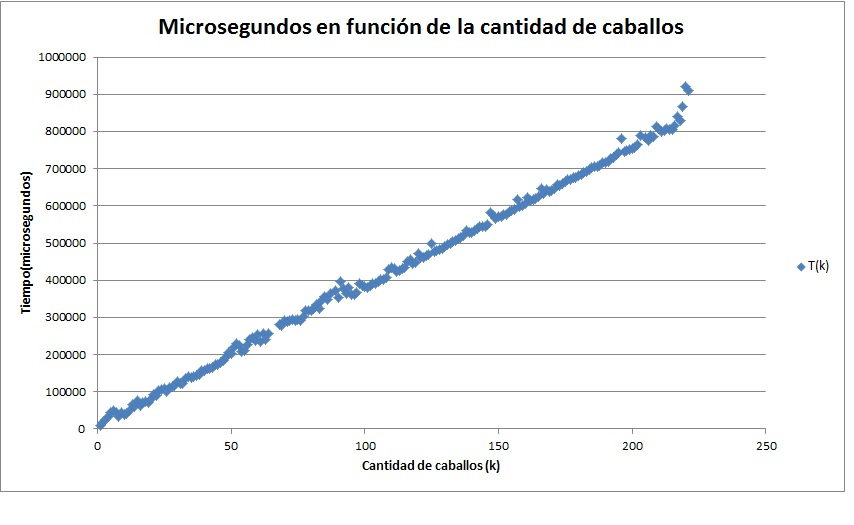
\includegraphics[scale=1]{Imagenes/Ej2/nFijo}
                \caption{T(k)=tiempo para k caballos }
                \label{fig:exp1}
\end{figure} 

Como podemos ver, obtuvimos una recta lo cual concluye al dejar constante n que la complejidad es O(k).\\

Veamos qué pasa cuando dejamos fija la cantidad de caballos en k=20 y variamos el tamaño del tablero (n) con una cantidad de 200 instancias:

\begin{figure}[H]
                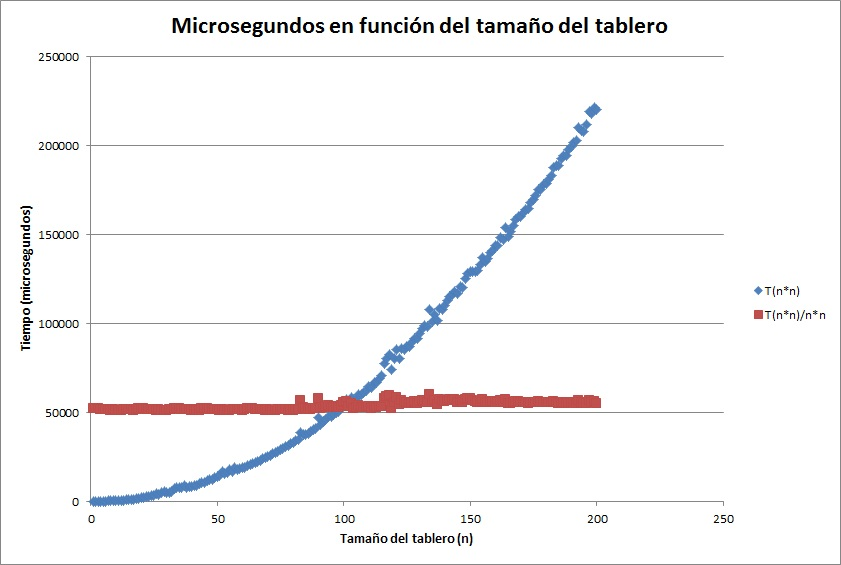
\includegraphics[scale=1]{Imagenes/Ej2/kFijo}
                \caption{T(n$^{2}$)=tiempo para tablero de tamaño n}
                \label{fig:exp2}
\end{figure} 
Como conclusión podemos ver que al dejar el k como una constante obtenemos una complejidad cuadrática del algoritmo contrastada en el gráfico.\\


Por ultimo una comparación cuando k y n varían de la misma manera con una cantidad de 300 instancias

\begin{figure}[H]
                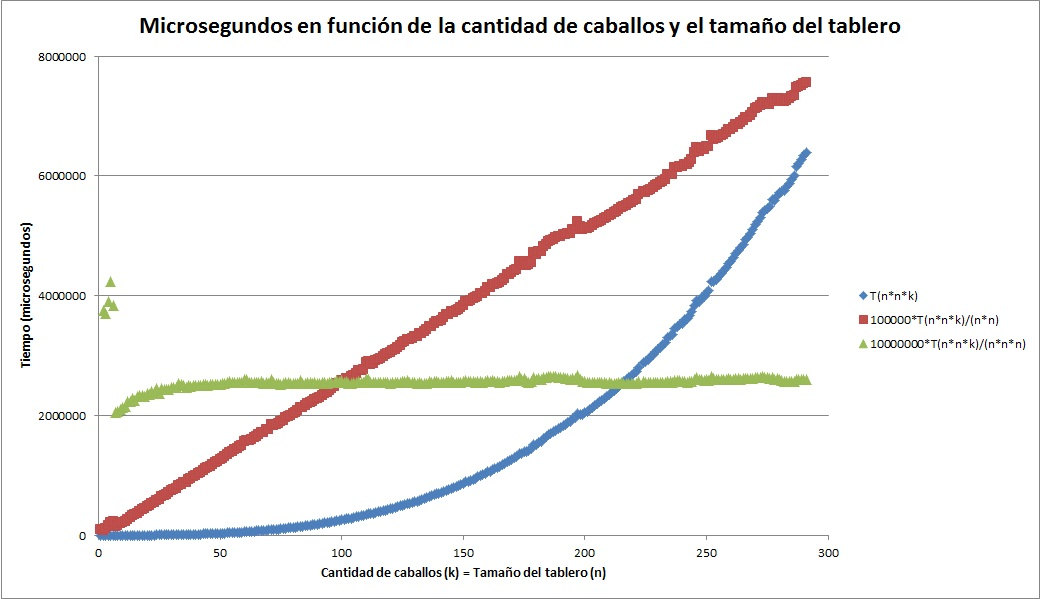
\includegraphics[scale=0.8]{Imagenes/Ej2/nkIguales}
                \caption{T(n$^{2}$*k)=tiempo para tablero de tamaño n = tiempo para k caballos}
                \label{fig:exp2}
\end{figure} 

En este último caso, se puede verificar una complejidad de O(n*$^{2}$*k)





\subsection{Conclusión}

Este ejercicio nos enseñó la posibilidad de utilizar algoritmos que a comienzo sirven para el recorrido de un grafo (BFS) como una manera de calcular caminos mínimos de grafos no pesados, o con todas las aristas del mismo peso. Con respecto al desarrollo, a priori no se nos presentó una dificultad al resolverlo, contamos con varias estrategias para encararlo, una de ellas era resolverlo con k matrices distintas para tener en cada matriz el camino mínimo a todas las casillas de un caballo nada más. Además pudimos cumplir con la complejidad que nos delimitaban y corroboramos empíricamente que el tiempo del algoritmo cumplía con esta.




	\newpage
	\section{Biohazard}

\subsection{Introducci\'on}
Este problema trata sobre transportar una cantidad  $n$ de productos químicos en camiones especiales para su traslado, sabemos que cada par de productos $p_{i}$ y $p_{j}$ reaccionan de distinta forma y por eso tiene un coeficiente de peligrosidad denominado $h_{ij}$. \\
Por normas de seguridad el nivel de peligrosidad de los productos transportados en un camión no puede superar un valor $M$, dicho nivel se mide de la siguiente manera:

$h(P) = \sum\limits_{\substack{
p_{i},p_{j} \epsilon P \\
i<j}} h_{ij}$ 


Nuestro objetivo es indicar como distribuir los productos químicos en los distintos camiones de forma de utilizar la menor cantidad de camiones posibles. \\ \\

A continuación un ejemplo del problema con su solución:


\begin{figure}[H]
  \centering
	\begin{subfigure}[b]{0.3\textwidth}
	
\begin{tabular}{| l | l |}
\hline
Cantidad de químicos:   & 2 \\ \hline
M:  & 20 \\ \hline
\end{tabular}


\begin{tabular}{| l | l | l |}
    \hline
    Peligrosidad Quimicos & 1 & 2 \\ \hline
    1 & 0 & 7 \\ \hline
    2 & 7 & 0 \\ \hline
\end{tabular}

	\end{subfigure} 
	\begin{subfigure}[b]{0.8\textwidth}

	 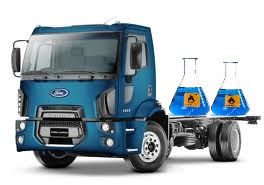
\includegraphics[scale=0.9]{Imagenes/Ej3/intro}
      
     \end{subfigure}
     \caption{Para este ejemplo los dos quimicos entran en 1 camion}
\end{figure}

\subsection{Desarrollo}


Para la resolución de este problema se no pidió que usáramos la técnica de Backtracking, por lo que nuestra idea del algoritmo comenzó por ir probando para cada producto químico todas las posibilidades de guardarlo en $n$ camiones (ya que como mucho metemos cada producto en un camión distinto), es decir la posibilidad de meter el químico $i$ al camión 1 y el resto de los químicos en distintos camiones, la posibilidad de meter los químicos $i$ y $j$ con $i$ != $j$ en el camión 1 y el resto en otros camiones, etc. Eventualmente nos quedamos con la posibilidad generada en la cual se usan menos camiones y no se supere el umbral $M$. \\
Luego pensamos podas y estrategias para mejorar al algoritmo, se nos ocurrieron las siguientes: 

\begin{itemize}
	\item Si probamos todas las posibilidades de distribuir los químicos en los distintos camiones con los químicos $i$ y $j$ con $i$ != $j$ en el camión 1, no vamos a probar lo mismo para el camión 2. Es decir, elimina todas las permutaciones en otros camiones de la misma solucion. \\
	Esta poda es buena en los casos donde hay muchos químicos que transportar pues entre más químicos hay, mas ramas de soluciones aparecen.
	
	\item Si en una rama del algoritmo tenemos un camión donde ya metimos $x$ productos químicos y al agregar un nuevo producto supera el umbral, entonces descartamos esa posibilidad. \\
	Esta estrategia es algo básica pero permite descartar ramas innecesarias las cuales no conducirán a una solución para el problema
 
\end{itemize}


\subsubsection{Pseudocódigo}

\LinesNumbered
\begin{algorithm}[H]
\DontPrintSemicolon
\KwData{\textbf{camiones}: conjunto de camiones, \textbf{productos}: conjunto de sustancias, \textbf{solucion}: conjunto de camiones}
\Begin{
	contador $\Leftarrow$ contar(camiones)\;
	\If{contador $ < $ minimosCamionesUsados} {

		\If{productos.todosUsados()} {
			minimosCamionesUsados $\Leftarrow$ contador \;
			solucion $\Leftarrow$ camiones \;
		}
		\For{ sust $\in$ productos } {
			\If{ $\not$ sust.usado() }  {
				\For{camion $\in$ camiones} {
					\If {(camion.noEsPeligroso(umbral, sust))} {
						camion.agregarSustancia(sust)\;
						Biohazard(camiones, productos, solucion)\;
						camion.sacarSustancia(sust)\;
					}
				}
			}
		}
	}
}
\caption{\textbf{Biohazard } \label{Biohazard }}
\end{algorithm}

La función contar, cuanta la cantidad de camiones utilizados. 
La función noEsPeligroso determina si agregar la sustancia al camión no supera el umbral.


\subsection{Complejidad}
Analicemos primero la naturaleza del problema. Tenemos n productos químicos los cuales tenemos que enviarlos a una fábrica mediante camiones. Nuestro objetivo es minimizar la cantidad de camiones contratados. Entonces podemos pensar un primer acercamiento en el cual comenzamos con n camiones. Esta va a ser nuestra solucion trivial, un camion por producto. A continuación probamos todas las maneras de distribuir los productos en estos camiones de manera tal que la cantidad de camiones contratados sea minima. Algo a resaltar es que un producto x pertenece a un camión nada mas (los productos son distinguibles). Entonces, cuantas maneras de distribuirlos tenemos?

Tenemos los productos $p_{1}$ $p_{2}$ y $p_{3}$. Pensemos esto como anagramas donde cada producto y camion es una letra. Sea $p_{i}$ la letra asociada al producto i y | la letra asociada al camion. Entonces lo que queremos buscar son la cantidad de anagramas que podemos formar con las letras $p_{1}$|$p_{2}$|$p_{3}$ en donde el orden de los camiones no nos importa. Si n = \# productos y m= \# camiones la formula sería:

$\frac{(n+m-1)!}{(m-1)!}$

En nuestro caso, m = n quedando

$\frac{(2n-1)!}{(n-1)!}$

Claramente la complejidad es exponencial.

Esta versión es nuestro algoritmo de backtracking sin ninguna poda. Ahora bien, algo importante a notar es lo siguiente: supongamos que tenemos 5 productos, y la distribucion optima es poner el producto $p_{1}$ $p_{2}$ y $p_{3}$ en un camion y el producto $p_{4}$ y $p_{5}$ en otro. Como nosotros partimos de tener n posibles camiones (en este caso serían 5), se solaparian las distribuciones donde $p_{1}$ $p_{2}$ y $p_{3}$ estan en el camion 1 mientras que los productos $p_{4}$ y $p_{5}$ en el camion 2 con las que esten $p_{1}$ $p_{2}$ y $p_{3}$ en el camion 2 con $p_{4}$ y $p_{5}$ en el camion 3. Entonces un segundo acercamiento sería sacar "`todas las permutaciones"' posibles de una distribucion dada (poda ya descripta). Esto sería lo mismo que contar los posibles subconjuntos de un conjunto cuyos elementos son los productos. Es decir, a nuestro caso $\{p_{1}, p_{2}\} = \{p_{2}, p_{1}\}$ quedando una complejidad de $O(2^n)$.

\subsection{Testing}

Decidimos tomar las siguientes instancias del problema para corroborar los resultados:\\

\textbf{Caso 1:} 2 productos químicos y el límite de peligrosidad 2. $h_{1,2}$ es 1.\\
\indent En este caso es obvio que ambos productos pueden viajar en 1 solo camión.

\textbf{Caso 2:} 3 productos químicos y el límite de peligrosidad 6. $h_{1,2} = 6, h_{1,3} = 7, h_{2,3} = 8$ .\\
\indent En un sólo camión no entran los 3 productos (tendría peligrosidad 21). Puedo poner el producto 1 y 2 en un camión, mientras que el 3 en otro camión. El mínimo en este caso es 2.

\textbf{Caso 3:} 3 productos químicos y el límite de peligrosidad 6. $h_{1,2} = 7, h_{1,3} = 7, h_{2,3} = 8$ .\\
\indent En este caso se puede ver que cada producto debe ir en camiones separados ya que la peligrosidad de a pares siempre supera el límite. En este caso el mínimo es 3.

\textbf{Caso 4:} 3 productos químicos y el límite de peligrosidad 8. $h_{1,2} = 2, h_{1,3} = 3, h_{2,3} = 3$ .\\
\indent En este caso se puede ver que todos los productos pueden viajar en un solo camión ya que la suma de sus peligrosidades es 8 y no supera el límite, que también es 8.\\

Estos casos de pruebas pueden encontrarse en \textbf{ej3/tester.cpp}.

\subsection{Experimentación}

Para los experimentos de medici\'on de tiempos decidimos armar un lote de entradas aleatorias, para generar dichas entradas, se utilizo un script en python al cual se le pasaban como par\'ametros los datos del problema y devolv\'ia valores pseudo-aleatorios.
A continuaci\'on haremos una comparaci\'on a nivel tiempo de ejecución de los algoritmos de backtracking con y sin podas, buscando confirmar que la versi\'on con podas 
tiene una mejora en el tiempo de ejecuci\'on. \\
También nos resultó interesante contrastar casos en donde la poda realizaba su mayor efecto. Comparamos (1) cuando necesitamos colocar una sustancia por camión debido a su alto indice de peligrosidad de a pares y (2) cuando podemos colocar todas las sustancias en un solo camión.

Grafico de (1)

\begin{figure}[h]
  \centering
    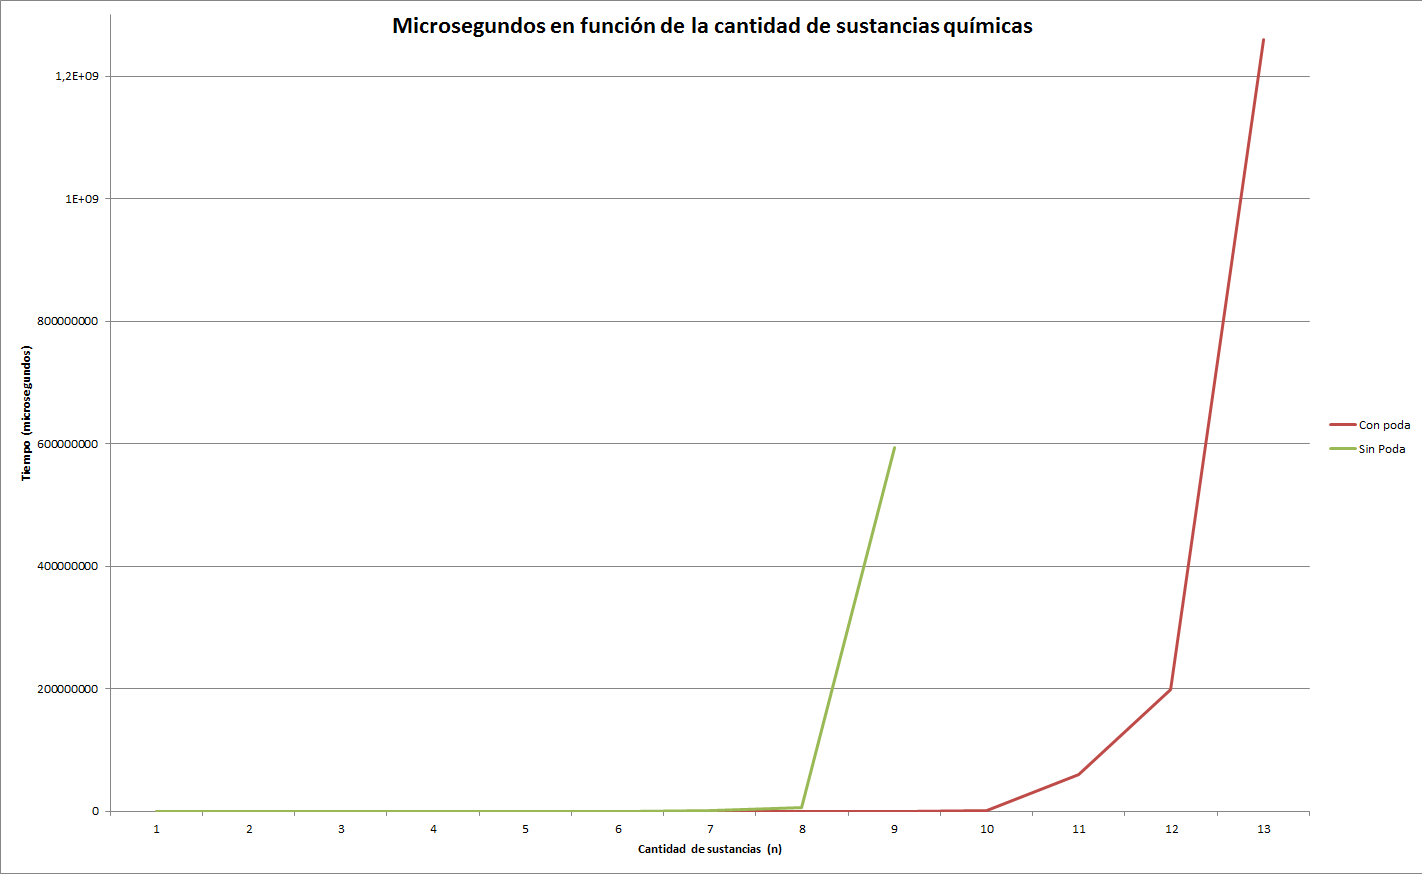
\includegraphics[scale=0.45]{Imagenes/Ej3/1solocamion.png}
  \caption{Una sustancia por camión}
  \label{fig:ejemplo}
\end{figure}

Grafico de (2)

\begin{figure}[h]
  \centering
    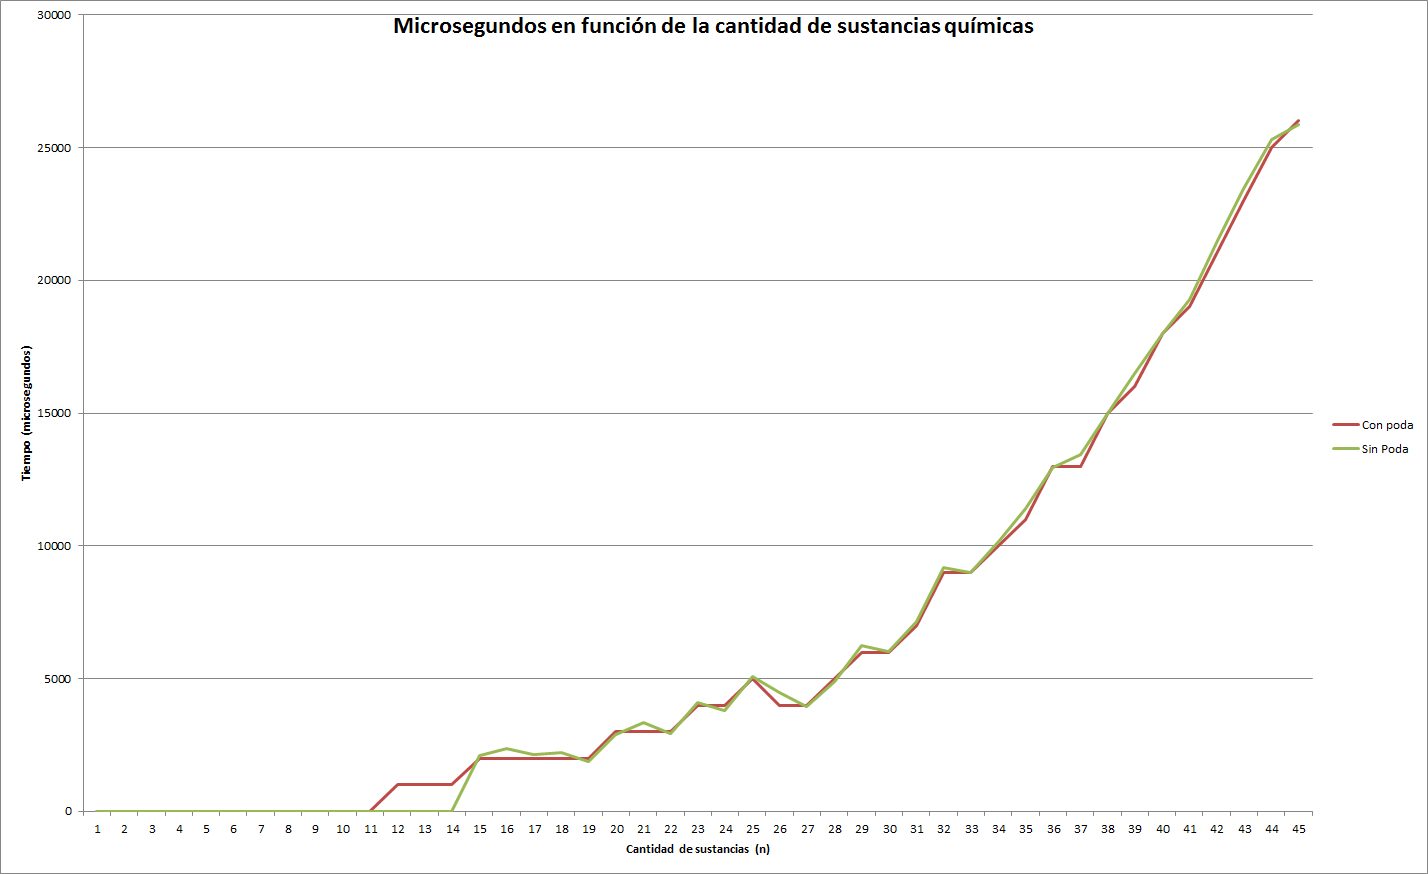
\includegraphics[scale=0.45]{Imagenes/Ej3/todo1camion.png}
  \caption{Todas las sustancias en un solo camión}
  \label{fig:ejemplo}
\end{figure}
	\newpage
	\appendix

\lstset{language=C++,
	basicstyle=\ttfamily\footnotesize,
	keywordstyle=\color{blue}\ttfamily,
	stringstyle=\color{red}\ttfamily,
	commentstyle=\color{green}\ttfamily,
	numbers=left,
	breaklines=true,
	tabsize=1,
	commentstyle=\color{magenta},
	morecomment=[l][\color{magenta}]{\#}
}


\section{Código fuente: Problema 1} \label{App:AppendixA}

\begin{frame}

\begin{lstlisting}
size_t dijkstra(size_t origen, size_t destino, adyacencias_t& adyacencias, std::list<size_t>& itenerario) {

    std::priority_queue< Tupla > cola;

    std::vector<size_t> distancia(ciudades_.size(), INFINITO);
    std::vector<size_t> padre(ciudades_.size(), INFINITO);
    std::vector<size_t> vuelo(ciudades_.size(), INFINITO);

    distancia[origen] = 0;
    cola.push(Tupla(origen, 0));

    while (!cola.empty()) {
        Tupla u =cola.top(); cola.pop();
        for(auto& v: adyacencias[u.first]) {
            if (distancia[v.des_] > v.fin_) {
                if ((distancia[u.first] == 0) || ((int)distancia[u.first] <= (int)(v.ini_ - 2))) {
                    distancia[v.des_] = v.fin_;
                    padre[v.des_] = u.first;
                    vuelo[v.des_] = v.id_;
                    cola.push(Tupla(v.des_, distancia[v.des_]));
                }
            }
        }
    }

    if (distancia[destino] != INFINITO) {
        size_t ciudad = padre[destino];
        itenerario.push_front(vuelo[destino]);
        while (ciudad != origen && ciudad != INFINITO) {
            itenerario.push_front(vuelo[ciudad]);
            ciudad = padre[ciudad];
        }
        // Si la ultima ciudad no es el origen, entonces no hay itinerario.
        if (ciudad == INFINITO) {
            itenerario.clear();
            return INFINITO;
        }
    }
    return distancia[destino];
}

\end{lstlisting}
\end{frame}

\newpage
\section{Código fuente: Problema 2} \label{App:AppendixB}

\begin{frame}

\begin{lstlisting}
class Tablero {
	/// Casillas
	int n_;
	/// Cantidad de caballos
	int k_;
	/// Casilla (f, c) elegida como destino final
	int f_;
	int c_;
	/// Cantidad de movimientos totales necesarios para llevar a todos los caballos a la casilla (f, c)
	int m_;
    
	typedef pair<int, int> coord_t;
	typedef vector<vector<int> > matriz_t;
	vector<coord_t> caballos_;

	inline bool esValido(const coord_t& c, int fila, int col) const {
		return ((c.first+fila <= n_) && (c.first+fila > 0) && (c.second+col <= n_) && (c.second+col > 0));
	}

	inline coord_t sumar(const coord_t& c1, const coord_t& c2) const {
		return coord_t(c1.first + c2.first,  c1.second + c2.second);
	}

	void dameAdyacentes(const coord_t& c, list<coord_t>& adyacentes) const {
		// movimiento de caballo arriba derecha
		if (esValido(c, 1, 2))
			adyacentes.push_back(sumar(c, coord_t(1, 2)));
		// movimiento caballo arriba izquierda
		if (esValido(c, -1, 2))
			adyacentes.push_back(sumar(c, coord_t(-1, 2)));
		// movimiento de caballo derecha abajo
		if (esValido(c, 2, -1))
			adyacentes.push_back(sumar(c, coord_t(2, -1)));
		// movimiento caballo derecha arriba
		if (esValido(c, 2, 1))
			adyacentes.push_back(sumar(c, coord_t(2, 1)));
		// movimiento caballo abajo derecha
		if (esValido(c, 1, -2))
			adyacentes.push_back(sumar(c, coord_t(1, -2)));
		// movimiento caballo abajo izquierda
		if (esValido(c, -1, -2))
			adyacentes.push_back(sumar(c, coord_t(-1, -2)));
		// movimiento caballo izquierda arriba
		if (esValido(c, -2, 1))
			adyacentes.push_back(sumar(c, coord_t(-2, 1)));
		// movimiento caballo izquierda abajo
		if (esValido(c, -2, -1))
			adyacentes.push_back(sumar(c, coord_t(-2, -1)));
	}

	void bfs(coord_t origen, matriz_t &m){
		queue<coord_t> cola;

		vector<bool> aux(n_, false);
		vector<vector<bool > > visitados(n_, aux);
		cola.push(origen);
		visitados[origen.first-1][origen.second-1]  = true;
		
		while(!cola.empty()){
			coord_t cab = cola.front(); cola.pop();

			list<coord_t> adyacentes;
			dameAdyacentes(cab, adyacentes);

			for(auto &v: adyacentes){
				if (visitados[v.first-1][v.second-1] == false){
					visitados[v.first-1][v.second-1] = true;
					m[v.first-1][v.second-1] = m[cab.first-1][cab.second-1] + 1;

					cola.push(v);
				}
			}
		}
	}


public:
	Tablero(): n_(0), k_(0), f_(0), c_(0), m_(numeric_limits<int>::max()) {}

	void resolver(){
		// Para acumular la cantidad de movimientos
		matriz_t acumMovimientos(n_, vector<int>(n_, 0));
		// Para contar si cada caballo pas\'o por cada posici\'on (tienen que estar los k).
		matriz_t cantidad(n_, vector<int>(n_, 0));

		// Ejecuto k bfs (para cada caballo)
		for(int cab = 0; cab < k_; ++cab) {
			matriz_t movimientos(n_, vector<int>(n_, 0));

			bfs(caballos_[cab], movimientos);

			// Una vez que termino el BFS, acumulo los movimientos.
			for (int i = 0; i < n_; ++i) {
				for (int j = 0; j < n_; ++j) {
					acumMovimientos[i][j] += movimientos[i][j];
					// Ahora verifico que el caballo haya estado en esta posici\'on
					if (movimientos[i][j] > 0)
						++cantidad[i][j];
					else {
						if ( (caballos_[cab].first-1 == i) && (caballos_[cab].second-1 == j))
							++cantidad[i][j];
					}
				}
			}
		}

		// Busco la casilla que tenga la m\'inima cantidad de movimientos y todos los caballos lleguen a esa casilla.
		m_ = numeric_limits<int>::max();
		for (int i = 0; i < n_; ++i) {
			for (int j = 0; j < n_; ++j) {
				if (cantidad[i][j] == k_) {
					if (acumMovimientos[i][j] < m_) {
						m_ = acumMovimientos[i][j];
						f_ = i+1;
						c_ = j+1;
					}
				}
			}
		}

	}

	void clear() {
		 f_ = 0;
		 c_ = 0;
		 m_ = numeric_limits<int>::max();
	}

	int size_n() const {
		return n_;
	}

	int size_k() const {
		return k_;
	}

};
\end{lstlisting}
\end{frame}

\newpage
\section{Código fuente: Problema 3} \label{App:AppendixC}

\begin{frame}

\begin{lstlisting}
class Nodo{
public:
    int numero, distancia;
    bool visitado, en_anillo;
    Nodo * padre;
    vector <pair <Nodo*, int> > adyacentes;
    vector <int> arista_en_AGM;

    Nodo(int numero, int N): numero(numero){
        padre = NULL;
        distancia = numeric_limits<int>::max();
        visitado = false;
        en_anillo = false;
        arista_en_AGM.resize(N+1);
    }

    void agregarAdyacente(Nodo* adyacente, int costo) {
        adyacentes.push_back(make_pair(adyacente, costo));
    }
};


struct Comp {
    bool operator()(const Nodo* s1, const Nodo* s2) {
        return (s1->distancia > s2->distancia);
    }
};

class LCdA{
public:
	int N, M, C;
	vector<Nodo> nodos;
    vector<pair < int , pair <Nodo*, Nodo* > > > aristas ;
    vector<pair<Nodo*, Nodo*> > anillo;
    vector<pair<Nodo*, Nodo*> > resto;

	LCdA():C(0){}
	int buscar_AGM() {
    
        // Si M < N no puede ser conexo y tener un ciclo
        if(M < N)
            return 1;

        vector <Nodo*>  heap;
        for (int i = 1; i <= N; i++)
            heap.push_back(&nodos[i]);

        Nodo * u = heap[0];
        u->distancia = 0;

        while (!heap.empty()) {   
            Nodo * u = heap.front(); pop_heap(heap.begin(), heap.end(), Comp()); 
            heap.pop_back();

            // Distancia es infinito <==> es no conexo
            if(u->distancia == numeric_limits<int>::max())
                return 1;

            // Anoto la arista como parte del AGM
            if (u->padre != NULL)        {
                u->arista_en_AGM[u->padre->numero] = 1;
                u->padre->arista_en_AGM[u->numero] = 1;
            }

            C+= u->distancia;
            u->visitado = true;

            for (unsigned int i = 0; i < u->adyacentes.size(); i++) {
                Nodo * v = u->adyacentes[i].first;
                if (!v->visitado && v->distancia > u->adyacentes[i].second) {
                    v->padre = u;
                    v->distancia = u->adyacentes[i].second;
                }
            }
            make_heap(heap.begin(), heap.end(), Comp());
        }
        return 0;
    }

	void formar_anillo() {
        sort(aristas.begin(), aristas.end());
        pair<Nodo*, Nodo*> arista_extra;

        for (unsigned int i = 0; i < aristas.size(); i++) {
            if(aristas[i].second.first->arista_en_AGM[aristas[i].second.second->numero] == 0) {
                C += aristas[i].first;
                arista_extra = aristas[i].second;
                break;
            }
        }

        Nodo * a = arista_extra.first;
        Nodo * b = arista_extra.second;

        // Formo el anillo llendo desde cada uno de los nodos de la arista extra hacia atras hasta llegar al otro nodo o a NULL
        for (int i = 0; i < 2; i++) {        
            while(a != NULL && a != b) {
                a->en_anillo = true;
                a = a->padre;
            }
            a = arista_extra.second;
            b = arista_extra.first;
        }

        anillo.push_back(arista_extra);

        // Separo las aristas del resto de las del anillo
        for (int i = 1; i <= N; i++) {
            Nodo* k = &nodos[i];
            if (k->padre != NULL) {
                if (k->en_anillo)
                    anillo.push_back(make_pair(k, k->padre));
                else
                    resto.push_back(make_pair(k, k->padre));
            }
        }
    }

};

\end{lstlisting}
\end{frame}


	\newpage
	\bibliographystyle{plain}
	\clearpage
	\bibliography{bibliography}
	\addcontentsline{toc}{section}{Referencias}
\end{document}

